\section{Measurements}\label{sec:results}

\S\ref{sec:pktest-results} holds the measurements of revision~2. Everything
before it is the historical measurement of revision~1, made on the
\art{crypto:eigen_seta/} build with the Mumford decapsulation chain. Those
numbers do not describe the maintained theta build.

All historical measurements were taken on one host: an Intel Xeon at 2.80\,GHz (shared
cloud VM, 4 logical cores), using rustc~1.97.0 in release mode. Two runs are
used. The benchmark run \art{run-20261011T1813Z-bench} used the code at
commit \art{19c641d12}. The verification run \art{run-20261011T1955Z-verify}
used commit \art{d504af28e}, which adds the key-generation checks and the
buffer wiping. The later commit \art{72051ac67} only caps the public
canonical-basis search; the known-answer tests confirm that it changes no
output. Their records are under
\art{crypto:research/eigen_seta_rust_20261011/reports/}.

\subsection{Sizes and speed}

\begin{table}[h]
\centering
\caption[Wall time per operation on one thread, as the range over trials
(trial count in brackets)]{Wall time per operation on one thread, as the range over trials
(trial count in brackets). Every decapsulation returned the encapsulated key.
Record: \art{run-20261011T1813Z-bench/records/bench_output.txt}.}
\label{tab:timings}
\begin{tabular}{lrrrr}
\toprule
set & pk = ct (B) & keygen (s) & encaps (s) & decaps (s)\\
\midrule
Toy16 & 216 & 0.38 [1] & 0.005--0.008 [5] & 0.12--0.19 [5]\\
Toy32 & 376 & 2.3 [1] & 0.009--0.012 [3] & 0.45--0.59 [3]\\
L1 & 1344 & 32.3 [1] & 0.24--0.26 [3] & 13.4--15.0 [3]\\
L3 & 1992 & 118.6 [1] & 1.03 [2] & 51.8--53.9 [2]\\
L5 & 2632 & 271.8 [1] & 2.17--2.20 [2] & 120.2--124.0 [2]\\
\bottomrule
\end{tabular}
\end{table}

\begin{figure}[h]
\centering
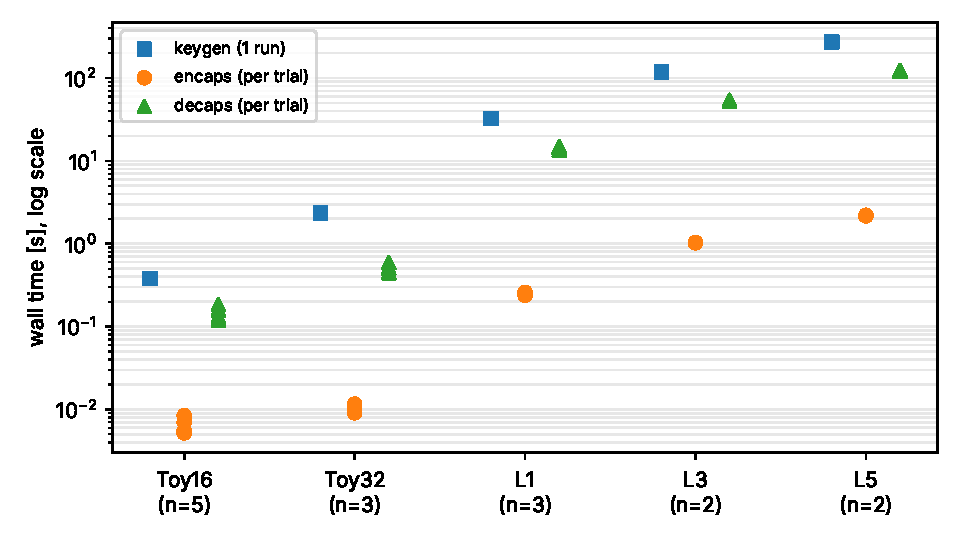
\includegraphics[width=0.78\textwidth]{figures/kem_times.pdf}
\caption[Wall time per operation, every trial shown, log scale]{Wall time per operation, every trial shown, log scale. Measured;
record as in Table~\ref{tab:timings}.}
\label{fig:times}
\end{figure}

Encapsulation is fast because it is a 3-isogeny chain of length $F$.
Decapsulation is dominated by the $E-6$ Richelot steps in Mumford
coordinates. Each step inverts a polynomial modulo a quartic for every point
it moves; from the formulas, we estimate a few hundred $\F_{p^2}$
multiplications per point and step. Key generation is a single sample, and
its time varies widely with the number of rejected candidates.

\begin{table}[h]
\centering
\caption[$\F_p$ arithmetic in ns per operation, in the same binary and run]{$\F_p$ arithmetic in ns per operation, in the same binary and run.
Multiplication is the minimum over 15 repetitions; inversion is the mean of
200. Record: \art{run-20261011T1813Z-bench/records/bench_output.txt}.}
\label{tab:field}
\begin{tabular}{lrrrr}
\toprule
set & limbs & mul & inversion, Fermat & inversion, safegcd\\
\midrule
Toy16 & 4 & 54 & 18,403 & 4,741\\
Toy32 & 6 & 72 & 67,657 & 10,316\\
L1 & 21 & 611 & 1,426,022 & 35,608\\
L3 & 32 & 1,516 & 6,708,390 & 109,506\\
L5 & 42 & 2,449 & 13,453,052 & 96,327\\
\bottomrule
\end{tabular}
\end{table}

No pre-change binary was kept as a baseline for the KEM-level timings, so we
claim no KEM-level speedup from the field optimisations.

\subsection{Correctness}

\begin{table}[h]
\centering
\caption[Decapsulation outcomes for honest ciphertexts with fresh OsRng keys
and ciphertexts]{Decapsulation outcomes for honest ciphertexts with fresh OsRng keys
and ciphertexts. Records:
\art{run-20261011T1955Z-verify/records/failrate/}, plus the benchmark run.}
\label{tab:failures}
\begin{tabular}{lrrl}
\toprule
set & trials & failures & record\\
\midrule
\FailRows
\bottomrule
\end{tabular}
\end{table}

Zero failures in 3,005 trials bounds the failure rate at Toy16 only by
about $10^{-3}$ at 95\% confidence (rule of three). The argument that the
rate is negligible is the heuristic $O(E/p)$ of \S\ref{sec:correctness};
the trials show that no systematic failure mode exists.

Beyond these, the known-answer tests and the robustness tests pass: 48
adversarial ciphertexts to decapsulation and 14 adversarial public keys to
encapsulation, with no panic and no hang (\art{crypto:eigen_seta/tests/}).

\subsection{Constant-time evidence}

Callgrind counted the instructions executed by \texttt{decaps\_core} alone,
with keys and ciphertexts generated from fixed seeds
(\art{crypto:eigen_seta/examples/ct_probe.rs}). The count splits into glibc's
allocator and \texttt{mem*} routines, whose work depends on heap layout but
not on secrets (\S\ref{sec:impl}), and everything else.

\begin{table}[h]
\centering
\caption[Instructions executed in the secret phase of decapsulation,
excluding glibc's allocator]{Instructions executed in the secret phase of decapsulation,
excluding glibc's allocator. ``Foreign'' ciphertexts are well formed but made
for another key, so the FO check rejects them. Records:
\art{run-20261011T1955Z-verify/records/toyprobe/ctprobe_summary.txt} and
\art{.../l1probe/ctprobe_summary.txt}.}
\label{tab:ct}
\begin{tabular}{lllr}
\toprule
set & keys & ciphertexts per key & non-allocator instructions\\
\midrule
\CTRows
\bottomrule
\end{tabular}
\end{table}

\begin{figure}[h]
\centering
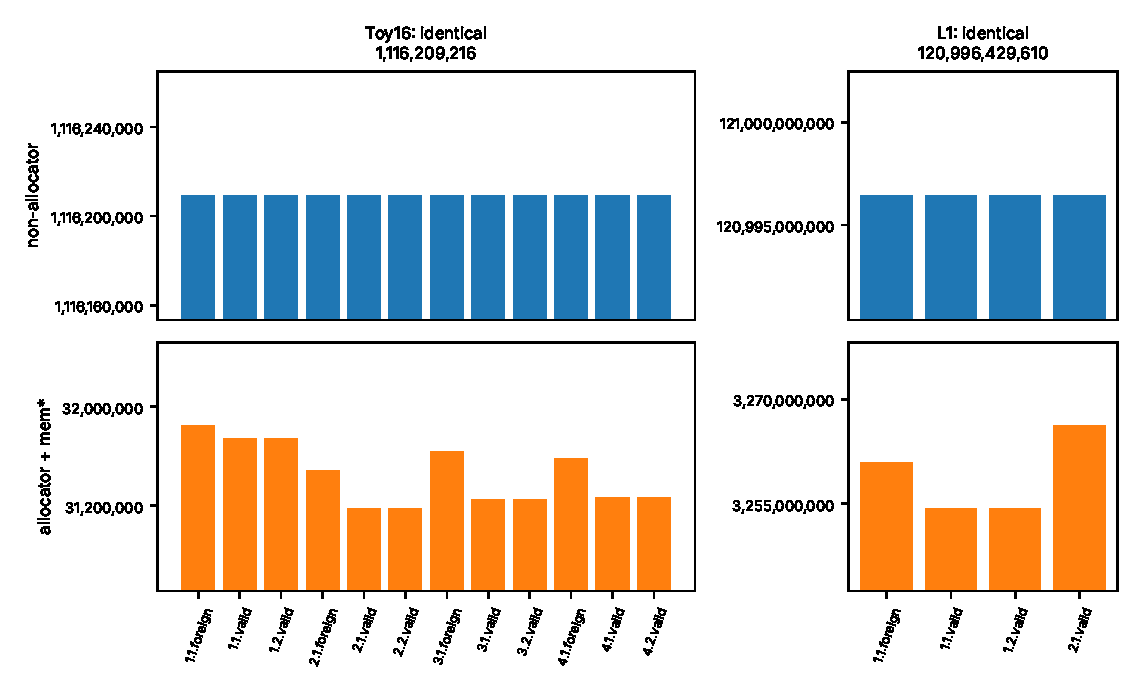
\includegraphics[width=0.78\textwidth]{figures/ct_probe.pdf}
\caption[Instruction counts of \texttt{decaps\_core} per run, at Toy16 (12
runs) and L1 (4 runs)]{Instruction counts of \texttt{decaps\_core} per run, at Toy16 (12
runs) and L1 (4 runs). Top: everything except glibc's allocator. Bottom:
glibc's allocator and \texttt{mem*}. Measured; records as in
Table~\ref{tab:ct}.}
\label{fig:ct}
\end{figure}

A statistical timing test in the style of dudect~\cite{RBV17}
(\art{crypto:eigen_seta/examples/dudect_decaps.rs}) used one Toy16 key and
interleaved two classes in random order: a fixed ciphertext and a pool of 16
fresh ones, half of them FO-rejected. With 1,000 samples per class, Welch's
statistic was \DudectT. The usual threshold for a detected leak is
$|t|>4.5$. This test is weaker than the instruction counts: it uses one key,
wall-clock time on a shared VM, and compares ciphertext classes rather than
keys. Record: \art{run-20261011T1955Z-verify/records/dudect_output.txt}.

\subsection{Revision 2: the public-key degree test}\label{sec:pktest-results}
Run \art{run-20261017T1623Z-pk-degree-test} executed
\art{eigenx:examples/pk_degree_test.rs} at \art{eigenx} commit
\art{94fe2d9} on a shared cloud VM (Intel Xeon at 2.10\,GHz, 4 logical
cores, rustc~1.97.0, release build, no core pinning). Records:
\art{crypto:research/eigen_seta_assessment_20261017/records/run-20261017T1623Z-pk-degree-test/}. For each
set it generates one key with its true $f$ and tests the true degree and a
number of wrong candidates with the theta chain of Lemma~\ref{lem:pktest}. A
candidate is accepted when the codomain is $\EA$. The wrong candidates are
uniform odd values prime to 21 and near misses $f+j2^k$ with
$k\in\{16,64,\lfloor\tfrac12\log_2f\rfloor\}$, $j\le4$. At L1 the true degree
and one wrong candidate were also walked with the structural checks of the
Mumford inspector. The true degree glued, ran all $e-6$ Richelot steps and
split exactly at the end. The wrong one glued, ran all steps with no early
split, and did not split.

\begin{table}[h]
\centering
\caption[Public-key degree test]{Public-key degree test. $e$ is the chain
length for the true degree, $e_{\min}=\lfloor\log_2 7f^2\rfloor+2$ is the shortest length the planner tries, and ``excess''
is the mean of $e-e_{\min}$ over the wrong candidates. The timings are the
median and range over interleaved repetitions of one test and one full
decapsulation of an honest ciphertext under the same key, wall time with
the crate's internal threads. Measured; record as above.}
\label{tab:pktest}
\small
\resizebox{\textwidth}{!}{%
\begin{tabular}{lrrrrrrr}
\toprule
set & $E$ & $e$ (true $f$) & $e_{\min}$ & excess & wrong (accepted) & test (s) & decaps (s)\\
\midrule
\PkRows
\bottomrule
\end{tabular}}
\end{table}

\begin{figure}[h]
\centering
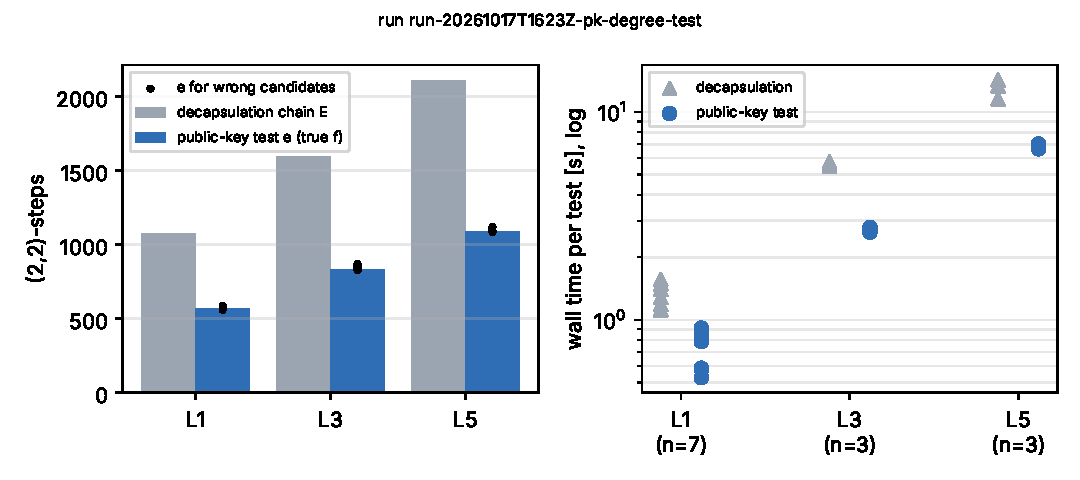
\includegraphics[width=0.78\textwidth]{figures/pk_test.pdf}
\caption[Public-key degree test against decapsulation]{Chain length (left)
and wall time per test (right) of the public-key degree test and of
decapsulation, every repetition shown. Measured; run \art{run-20261017T1623Z-pk-degree-test}.}
\label{fig:pktest}
\end{figure}

The chain is $e/E\approx0.52$ of the decapsulation chain at every set,
because $e\approx2\log_2f$ and $E\approx4\log_2f$. The ratio of the median
times is 1.6 at L1 and 2.0 at L3 and L5. Decapsulation also pays for
ladders, pairings and the re-encryption. The L1 ranges overlap less
cleanly, and we do not explain the lower ratio there. These timings are on a noisy shared
VM and support only the factor-of-two reading. The cost model's gate
columns for the degree search drop by $1.9$ bits as a result. This changes
no tier, because the degree search is far from binding.

